\documentclass[12pt,a4paper]{report}
\usepackage[utf8]{inputenc}
\usepackage{amsmath}
\usepackage{amsfonts}
\usepackage{amssymb}
\usepackage{graphicx}
\usepackage{enumitem}
\usepackage{dsfont}
\usepackage[left=2cm, right=2cm, top=4cm, bottom=2cm]{geometry}

\begin{document}
	\begin{titlepage}
		\centering
		{\scshape\LARGE Universidad Nacional Autónoma de México \par}
		\vspace{1cm}
		{\scshape\Large Probabilidad I\par}
		\vspace{1.5cm}
		{\huge\bfseries Tarea IV\par}
		\vspace{.5cm}
		{\Large\itshape Sandra Del Mar Soto Corderi \par}
		\vspace{.5cm}
		{\Large\itshape Edgar Quiroz Castañeda \par}
	    \vspace{.5cm}
		{\Large\itshape Raúl Llamosas Alvarado \par}
		 \vspace{.5cm}
		{\Large\itshape Alan Ernesto Arteaga Vázquez \par}
		 \vspace{.5cm}
		{\Large\itshape Jean Paul \par}
		\vfill
		 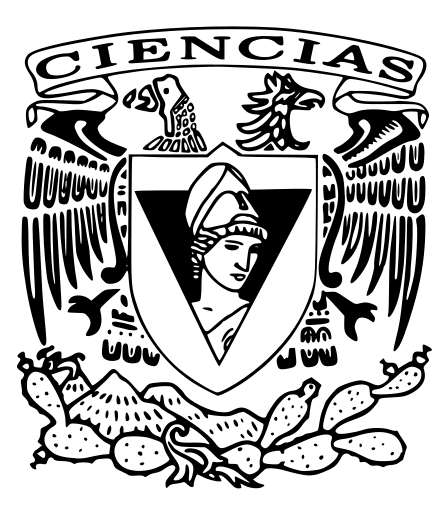
\includegraphics[width=0.5\textwidth]{escudo.png}
		\vfill

		{\large Martes 15 de octubre del 2018 \par}
	\end{titlepage}

	\pagebreak
	\setlength{\voffset}{-0.75in}
	\setlength{\headsep}{5pt}

	\begin{enumerate}
  
		%Ejercicio 1
		\item {
			Sea $A$ un evento $(A \in F)$. Definimos $X$ por
			\[
				X(\omega) =
				\begin{cases}
					1, $ si $\omega \in A\\
					0, $ si $\omega \not\in A
				\end{cases}
			\]
      
			¿Es $X$ variable aleatoria?\\
			
			Tenemos que una variable aleatoria está definida como: \\
			\textbf{Definición:} Para un espacio de probabilidad $P=(\Omega,F,P)$ tenemos que $X:\Omega \mapsto \mathds{R}$ es una variable aleatoria si:
        		   	\begin{center}
			   $ \lbrace w\in \Omega : X(w) \leq x \rbrace \in F.$
			\end{center}
			Donde $x\in \mathds{R}$ y $Im^{-1}(X)=(-\infty,x]$. Tenemos que la función está dada para un evento en específico de A. Si F está dado como: \\
			\begin{center}
			    $F= \lbrace A, A_{1},...,A_{n} \rbrace \subset P(\Omega): \Omega = \lbrace O_{1},...,O_{k} \rbrace $
			\end{center}
			Tenemos que los valores de la función está acotada por 1 y por 0. Entonces los rangos de x corren en $(-\infty,0),[0,1),[1,\infty)$. Tenemos entonces que:\\
		    \begin{center}
		        si $x\in (-\infty,0) \Rightarrow \lbrace w \in \Omega: X(w) \leq x \rbrace =  \emptyset  \in F $\\
		        si $x\in [0,1)  \Rightarrow \lbrace w \in \Omega: X(w) \leq x \rbrace = \lbrace w\in \Omega : X(w)=0 \rbrace$
		    \end{center}
		    Pero ésto solamente sucede cuando $w\notin A $, es decir cuando $w \in A^c$, pero como F es una $\sigma-algebra$ entonces claramente $A^c\in F$ por lo que $\lbrace w \in \Omega : X(w) \leq x \rbrace = A^c \in F$ si $x\in [0,1)$.  Ahora tenemos que si:\\
		    \begin{center}
		        si $x\in [1,\infty) \Rightarrow \lbrace w \in \Omega : X(w) \leq x \rbrace = \lbrace w \in \Omega : X(w)=1 \rbrace  = \lbrace w\in \Omega: w \in A \rbrace = A$. 
		        Y $A \in F$ por hipótesis. Entonces cumple los requisitos de que sea una variable aleatoria$_{\blacksquare}$
		    \end{center}
					
		%Ejercicio 2

		\item {
			Considere un espacio de probabilidad $\Omega = \{1, 2, 3, 4, 5, 6\}$ y
			$F = \{\emptyset, \Omega, \{2, 4, 6\}, \{1, 3, 5\}\}$.\\
			Sean $X_1, X_2 : \Omega \rightarrow \mathbb{R}$ definidas como
			\begin{align*}
				X_1(\omega) = \omega^2 & X_2(\omega) = \begin{cases}
																								1, \omega $ par$\\
																								0, \omega $ impar$
																							\end{cases}
			\end{align*}
			¿Son $X_1$ y $X_2$ variables aleatorias en este espacio de probabilidad?
			Tenemos que: \\
			\begin{center}
			    $X_{1}(w)= \begin{cases} 1, si\ \omega=1\\ 4,si \ \omega=2 \\ 9, si \ \omega=3\\ 16, si \ \omega=4 \\ 25, si \ \omega=5 \\ 36, si \ \omega=6  \end{cases}$
			\end{center}
			Entonces que los intervalos a considerar son $(-\infty,1),[1,4),[4,9),[9,16),[16,25),[25,36),[36,\infty)$\\
			\begin{center}
			    si $x\in (-\infty,1) \Rightarrow \lbrace w\in \Omega : X(w)\leq x \rbrace = \emptyset \in F $ \\ 
			    si $x\in [1,4) \Rightarrow \lbrace w \in \Omega : X(w) \leq x \rbrace = \lbrace 1 \rbrace \notin F$
			\end{center}
			Como podemos ver, no se encuentra en F por lo tanto  $X_{1}$ no es una variable aleatoria. Ahora, tenemos que:\\
			\begin{center}
			    $X_{2}(w) = \begin{cases}
			    1, si \ \omega \in \lbrace 2,4,6 \rbrace \\
			    0, si \ \omega \in \lbrace 1,3,5 \rbrace 
			    \end{cases}$
			\end{center}
			}
			Los intervalos a considerar son $(-\infty,0),[0,1),[1,\infty)$ entonces:\\
			\begin{center}
			    si $x\in (-\infty,0) \Rightarrow \lbrace w\in \Omega: X(w) \leq x \rbrace = \emptyset \in F. $\\
			    si $x\in [0,1) \Rightarrow \lbrace w \in \Omega: X(w) \leq x \rbrace = \lbrace 1,3,5 \rbrace \in F$  \\
			    si $x\in [1,\infty) \Rightarrow \lbrace w\in \Omega: X(w)\leq x \rbrace = \lbrace 2,4,6 \rbrace \in F$
			\end{center}
		    Entonces sí es una variable aleatoria. Entonces en conclusión $X_{2}$ es una variable aleatoria pero $X_{1}$ no lo es.
		}
		
		%Ejercicio 3		
		\item {
			Sea $f$ una función definida por
			\[
				f(x) = \begin{cases}
								x+1, $ si $ -1 \leq x \leq 0\\
								2x-6, $ si $ 3 \leq x \leq c\\
								0, $ en otro caso$
			\end{cases}
			\]
			Con $c$ constante.
			\begin{enumerate}
				\item{
					Determine el valor de $c$ de tal manera que $f$ sea una función de
					densidad.
					
					
					Como es una función de densidad continua tenemos que tiene que cumplir lo siguiente:
					\begin{center}
					    $$\int_{-\infty}^{\infty} f(x) dx = \int_{-\infty}^{-1}f(x)dx+\int_{-1}^{0}f(x)dx+\int_{0}^{3}f(x)dx+\int_{3}^{c}f(x)dx+\int_{c}^{\infty}f(x)dx$$\\
					    $$=0+\int_{-1}^{0}(x+1)dx+0+\int_{3}^{c}(2x+6)dx+0=$$\\ 
					    $$(\frac{x^2}{2}+x)|_{-1}^{0}+2[(\frac{x^2}{2}+3x)|_{3}^{c}]=1$$\\
					    $$(\frac{0^2}{2}+0)-(\frac{(-1)^2}{2}-1)+2[(\frac{c^2}{2}+3c)-(\frac{9}{2}+9)]=1$$ \\
					    $$\frac{1}{2}+2[(\frac{c^2+6c}{2})-(\frac{27}{2})]=1$$\\ 
					    \end{center}
					 Y eso solo sucede cuando: 
					\begin{center}
					    $$c^2+6c-27+\frac{1}{2}=1$$\\
					    $$c^2+6c-\frac{55}{2}=0$$
					\end{center}   
					Cuyos valores que resuelven dicha ecuación son:\\
					\begin{center}
					    $c_{1}=\frac{-6+\sqrt{36+110}}{2}=\frac{-6+\sqrt{146}}{2}$\\
					    $c_{2}=\frac{-6-\sqrt{146}}{2}$
					\end{center}
					Tenemos que el valor tendría que ser positivo para que ésto tuviese sentido y dado que $c_{1}\approx 3.041 $ se tiene que éste será el valor que tenga que tomar c. Entonces el valor de c es:
					\begin{center}
					   $$ c=\frac{-6+\sqrt{146}}{2}$$
					\end{center}
				    }
				
				\item {
					Encuentre la función de distribución correspondiente a $f$.\\ \\
					Al tratarse de una función continua se tiene que $F(x)= \int_{-\infty}^{x} f(t)dt$ entonces se sigue que:\\
					\begin{center}
					    $F(x)= \begin{cases} 
					    \frac{x^2}{2}+x, \ $si$ \ -1\leq x \leq 0 \\
					    \frac{3x^2}{2}-5x, \ $si$ \ 3\leq x \leq  \frac{-6+\sqrt{146}}{2}
					    
					    \end{cases}$
					\end{center}
					Ya que que al tratarse de una función acumulativa se suma a la integral  $\int 2x-6$ la integral $\int x+1$ debido a que es acumulativa. 
					
					
				}
			\end{enumerate}
		}
		
		%Ejercicio 4
		\item {
			Sea $f$ una función definida por
			\[
				f(x) = \begin{cases}
								cr^x, $ si $ x \in \{0, 1, ...\}\\
								0, $ en otro caso$
							 \end{cases}
			\]
			En donde $0 < r < 1$. Encuentre $c$ para que $f$ sea función de densidad.
		}
		
		%Ejercicio 5
		\item {
		La función de densidad de una variable aleatoria $X$ es
		\[f_X(x) = \gamma x^2 e^{-kx}\mathbb{I}_{(0, \infty)}\]
		Donde $k > 0$.
		\begin{enumerate}
			\item {
				Encontrar el valor de $\gamma$.
			}
			\item {
				Encontrar la función de distribución $F_X$ de la variable aleatoria
				$X$.
			}
			\item {
				Calcule $P(0 < X < \frac{1}{k})$
			}
		\end{enumerate}
		}
		
		%Ejercicio 6
		\item {
			Sea
			\[
				f(x) = \begin{cases}
								0, $ si $ x < 0\\
								\frac{1}{2}\beta, $ si $ 0 \leq x < 1\\
								\frac{1}{2}, $ si $ 1 \leq x < 2\\
								\frac{1}{2}(1-\beta), $ si $ 2 < x < 3\\
								0, $ si $ x \geq 3
						 	 \end{cases}
			\]
			Donde $0 < \beta < 1$. Encontrar la función de distribución $F_X$
		}
		
		%Ejercicio 7
		\item {
			Demuestre que $f_X(x) = \frac{1}{2}e^{-|x|}\mathbb{I}_\mathbb{R}(x)$ es
			una función de densidad.
		}
		
		%Ejercicio 8
		\item {
			Sea $X$ una variable aleatoria con función de densidad
				\[f_\gamma(y) = cy \mathbb{I}_{\{1, 2, 3, 4\}}(y)\]
				\begin{enumerate}
					\item {
						Determinar el valir de $c$ para que $f_\gamma$ sea una función de
						densidad de probabilidad.
					}
					\item {
						Calcule $P(1 < Y \leq 3)$ y $p(Y < 1 | Y \leq 3)$
					}
				\end{enumerate}
		}
		
		%Ejercicio 9
		\item {
			Sea $X$ una variable aleatoria continua con función de densidad
				\[
					f_X(x) = \begin{cases}
										6x(1-x), $ si $ 0 < x < 1\\
										0, $ en otro caso$
									 \end{cases}
				\]
			Calcule $P(|X-\frac{1}{2}| > \frac{1}{4})$.
		}
		
		%Ejercicio 10
		\item {
			Suponga que se selecciona aleatoriamente un punto $z$ del cuadrado con
			esquinas (2, 1), (3, 1), (2, 2,) y (3, 2). Sea $A$ la variable aleatoria
			que mide el área del triángulo con vértices (2, 1), (3, 1) y $z$.
			\begin{enumerate}
				\item {
					¿Cuál es el valor más grande que $A$ puede tomar?
				}
				\item {
					¿Cuál es el conjunto de puntos para el cuál $A \leq \frac{1}{2}$?
				}
				\item {
					Encuentre la función de densidad de $A$.
				}
				\item {
					Encuentre la función de distribución de $A$.
				}
			\end{enumerate}
		}
		
		%Ejercicio 11
		\item {
			Una póliza de seguros cubre las reclamaciones médicas de los empleados
			de una pequeña compañía.\\
			El valor $V$ de las reclamaciones hechas en un año es descrita mediante
			\[V = 100000Y\]
			Donde $Y$ es una variable aleatoria con función de densidad
			\[
				f_\gamma(y) = \begin{cases}
												k(1-y)^4, $ si $ 0 < y < 1\\
												0, $ en otro caso$
											\end{cases}
			\]
			Donde $k$ es constante. ¿Cuál es la probabilidad de que $V$ exceda 10000?
			}
			
		%Ejercicio 12
		\item {
			Una urna contiene 5 bolas rojas y 5 bolas azules. Se realiza un juego
			que consiste en extraer aleatoriamente 2 bolas de la urna. Suponga que
			si se extraen dos bolas del mismo color, el jugador gana \$1.11 y si se
			extraen dos bolas de distinto color el jugador pierde \$1.00. Si una
			persona participa en el juego dos veces, calcule la probabilidad de que
			la ganancia de esta persona sea mayos a \$0.00.
		}

		%Ejercicio 13		
		\item {
			Sea $X$ una variable aleatoria con función de densidad dada por
			\[f_X(x) = \frac{1}{2}e^{-|x|}\mathbb{I}_{\mathbb{R}}(x)\]
			Si $Y = X^2$, encuentre la función de distribución acumulada de $Y$.
			
			Para obtener la función de distribución acumulada usamos la ley de estadística inconsciente y tenemos que:
			
		$F_{x}(y) = P(Y \leq y) = P(X^2\leq y) = P(-\sqrt{y} \leq X \leq \sqrt{y})$	\\
					
			Ya que es una variable aleatoria continua, y basándonos en cómo definimos la función de distribución arriba, el resultado sería la siguiente integral:
			$\int_{-\sqrt{y}}^{\sqrt{y}} \frac{1}{2}e^{-|x|}$			
			
			Desarrollamos:
			 \[
               \int_{-\sqrt{y}}^{\sqrt{y}} \frac{1}{2}e^{-|x|}
                =
                 \int_{-\sqrt{y}}^{0} \frac{1}{2}e^{x} 
                 +
                 \int_{0}^{\sqrt{y}} \frac{1}{2}e^{-x}
                =
                 \left[\frac{1}{2}e^{x}\right]\Big|_{-\sqrt{y}}^{0}
                 +
                 \left[-\frac{1}{2}e^{-x}\right]\Big|_{0}^{\sqrt{y}}
             \]        
             \[
                           =
                \left(\frac{1}{2} - \frac{1}{2}e^{-\sqrt{y}}\right)
                +
                \left(- \frac{1}{2}e^{-\sqrt{y}} + \frac{1}{2}\right)
                =
                1 - e^{-\sqrt{y}}
            \]        
            
            De ahí,\\
            $F_{x}(y) =  1 - e^{-\sqrt{y}}$\\
		}
		
		%Ejercicio 14
		\item {
			Sea $X$ una variable aleatoria con función de densidad dada por
			\[
				f_X(x) = \begin{cases}
									4x^3, $ si $ 0 < x < 1\\
									0, $ en otro caso$
								 \end{cases}
			\]
			Encuentre $P(X \leq \frac{2}{3}|X > \frac{1}{3})$.\\
			
			Tenemos una probabilidad condicional y vemos que:\\
			
			 $P(X \leq \frac{2}{3}|X > \frac{1}{3}) = \frac{P((X \leq \frac{2}{3}) \cap (X > \frac{1}{3}))}{P(X > \frac{1}{3})}$\\
			 
			 Sabemos que la variable es continua, y estamos evaluando en el caso donde está entre $ 0 < x < 1$ ya que es el caso donde está valuada,  así que:\\
			 
			 $P((X \leq \frac{2}{3}) \cap (X > \frac{1}{3})) = \int_{\frac{1}{3}}^{\frac{2}{3}} 4x^3 dx$ \\
			 
			 Ya que en el caso donde estamos valuando, el límite está en 1, podemos tener lo siguiente:
			 $P(X > \frac{1}{3}) = \int_{\frac{1}{3}}^{1} 4x^3 dx$\\
			 
			 Desarrollamos:\\
			 $P((X \leq \frac{2}{3}) \cap (X > \frac{1}{3})) = 
			 \left[x^4\right]\Big|_{\frac{1}{3}}^{\frac{2}{3}}=
			 \frac{16}{81} - \frac{1}{81} = \frac{5}{27}$\\
			 
			 $P(X > \frac{1}{3}) = 
			 \left[x^4\right]\Big|_{\frac{1}{3}}^{1}=
			 1 - \frac{1}{81} = \frac{80}{81}$\\
			 
			 Entonces,\\
			 $P(X \leq \frac{2}{3}|X > \frac{1}{3})
			 = \frac{\frac{5}{27}}{\frac{80}{81}}
			 = \frac{3}{16}$
			 
			 
			 
			 
		}
	\end{enumerate}
\end{document}